% HEADER
\documentclass[class=article, crop=false]{standalone}
\usepackage{00_Preamble/frr_preamble}

% Packages
\usepackage{titlesec}
\usepackage{hyperref}
\usepackage{float}
\usepackage{graphics}
\usepackage{placeins}
\usepackage{adjustbox}
% END HEADER

\begin{document}
	\subsection{Purpose of Systems Engineering}
	\label{subsec:systems_engineering_purpose}
	The Vanderbilt Robotics Team followed a systems engineering design process outlined by the V-chart presented in Figure \ref{fig:safety_protocol_flowsheet}. The excavation robot has many conflicting constraints and multiple subsystems that all need to perform equally well in order to accomplish the presented challenge. The systems engineering process provides a structured methodology to optimize competing requirements and available resources. It provides a holistic, big-picture approach to the decision making process. 
	
	\FloatBarrier
		\begin{figure}[h]
			\centering
			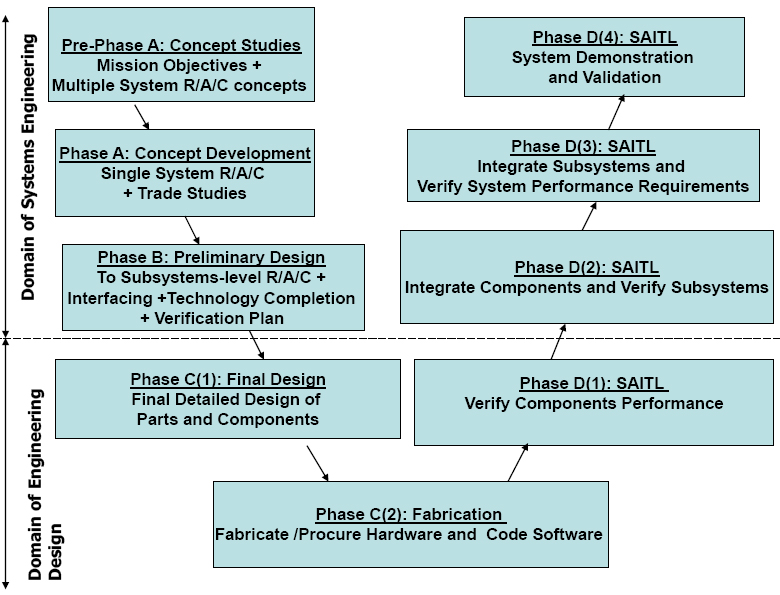
\includegraphics[width=.50\linewidth]{09_Figures/systems_engineering_vee_chart.jpg}
			\caption{Systems Engineering Vee Chart}
			\label{fig:safety_protocol_flowsheet}
		\end{figure}
		\FloatBarrier


	
\end{document}
